\chapter{開弦の量子からタキオンと重力へ}

\lectureoverview{ここでは前回の講義で求めた正常モードを量子化し、それらがどのような粒子状態を生み出すかを問う。各横モードは調和振動子であるが、その規格化はやや馴染みが薄い。モード\(n\)を励起すると、光円錐エネルギーが、したがって質量二乗の準位が、\(n\)単位だけ上がる。最初の励起開弦準位は、質量ゼロのベクトルの二つの横偏極と全く同じように変換する。したがって相対論的整合性により、基底状態の質量二乗は負でなければならない。その状態がボソン弦のタキオンであり、その真の意義は不安定な真空であって、実用的な超光速粒子ではない。最後に、弦が相互作用すると、結合と分裂により閉弦は避けられなくなる。最低次の閉弦励起が重力子となる。}

\section{各弦モードに隠れた振動子}

一つの横座標\(X\)に対し、\(n\)番目の非零正常モードはエネルギーとラグランジアン

\begin{align}
  E_n
  &=
  \frac14\dot X_n^{\,2}
  +\frac{n^2}{4}X_n^2,
  \label{eq:l03-mode-energy}\\
  L_n
  &=
  \frac14\dot X_n^{\,2}
  -\frac{n^2}{4}X_n^2.
  \label{eq:l03-mode-lagrangian}
\end{align}

\(1/4\)の因子は誤りではない。それらは弦の作用が独立なフーリエモードに還元されたときに選ばれた規格化を記録している。したがってハミルトニアンを構成する第一歩は、正準運動量を計算することである。

\begin{equation}
  p_n=\frac{\partial L_n}{\partial\dot X_n}
     =\frac12\dot X_n,
  \qquad
  \dot X_n=2p_n.
  \label{eq:l03-canonical-momentum}
\end{equation}

ルジャンドル変換により

\begin{equation}
  H_n=p_n\dot X_n-L_n
     =p_n^2+\frac{n^2}{4}X_n^2.
  \label{eq:l03-mode-hamiltonian}
\end{equation}

\begin{figure}[H]
  \centering
  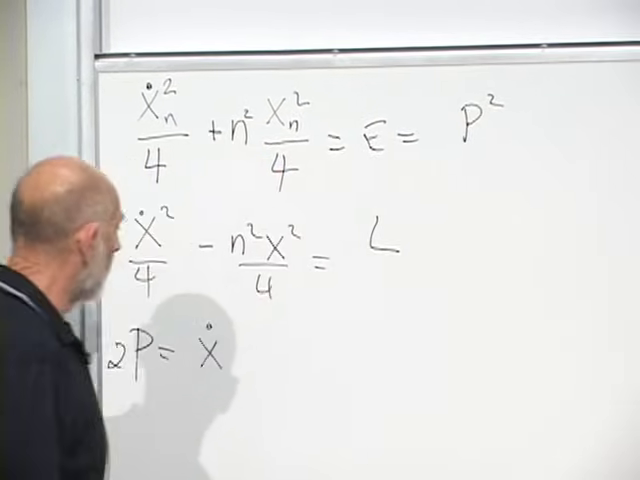
\includegraphics[width=0.82\textwidth]{lecture_03_figure_01.png}
  \caption{開弦から受け継いだ規格化におけるモードのエネルギー、ラグランジアン、正準運動量、ハミルトニアン。}
  \lectureframe{00:05:40}
  \label{fig:l03-mode-hamiltonian-board}
\end{figure}

\(H_n\)を因数分解するには、\(X_n\)と\(p_n\)を次のように組み合わせる。

\begin{equation}
  \frac{nX_n}{2}\pm i p_n.
\end{equation}

古典的には二つの因子は可換であるが、量子力学的には

\begin{equation}
  [X_n,p_m]=i\delta_{nm}
  \label{eq:l03-canonical-commutator}
\end{equation}

\(\hbar=1\)の単位で。交差項は無害には相殺しない。固定されたモードに対して、

\begin{align}
  \left[\frac{nX_n}{2}+ip_n,
        \frac{nX_n}{2}-ip_n\right]
  &=n,
  \label{eq:l03-unscaled-commutator}\\
  \left(\frac{nX_n}{2}-ip_n\right)
  \left(\frac{nX_n}{2}+ip_n\right)
  &=H_n-\frac n2.
  \label{eq:l03-factorized-hamiltonian}
\end{align}

\begin{figure}[H]
  \centering
  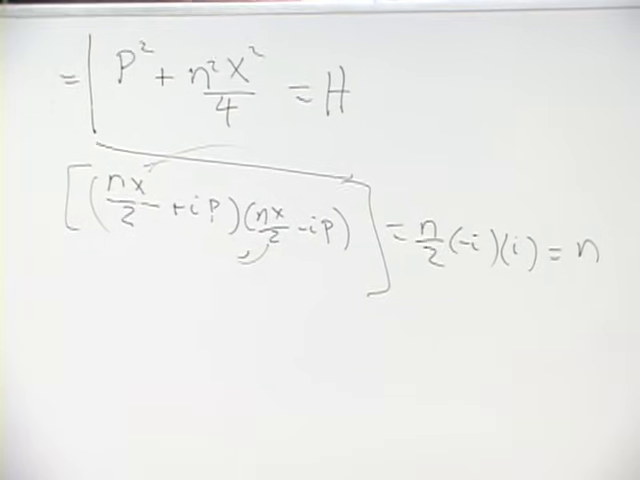
\includegraphics[width=0.82\textwidth]{lecture_03_figure_02.png}
  \caption{正準交換子が\(n\)の因子を与える板書計算。}
  \lectureframe{00:10:30}
  \label{fig:l03-commutator-board}
\end{figure}

\(n\)の因子は、はしご演算子をどのように規格化すべきかを教えてくれる。

\begin{align}
  a_n
  &\equiv
  \frac{\sqrt n}{2}X_n+\frac{i}{\sqrt n}p_n,
  \label{eq:l03-annihilator}\\
  a_n^\dagger
  &\equiv
  \frac{\sqrt n}{2}X_n-\frac{i}{\sqrt n}p_n.
  \label{eq:l03-creator}
\end{align}

それらは次を満たす。

\begin{equation}
  [a_n,a_m^\dagger]=\delta_{nm},
  \qquad
  H_n=n\left(a_n^\dagger a_n+\frac12\right).
  \label{eq:l03-oscillator-algebra}
\end{equation}

したがって\(a_n^\dagger\)は\(n\)番目の振動子の量子を一つ加えるが、その量子は\(n\)単位のモードエネルギーを運ぶ。お馴染みの振動子間隔は失われていない。その振動数は\(\omega_n=n\)である。

\begin{figure}[H]
  \centering
  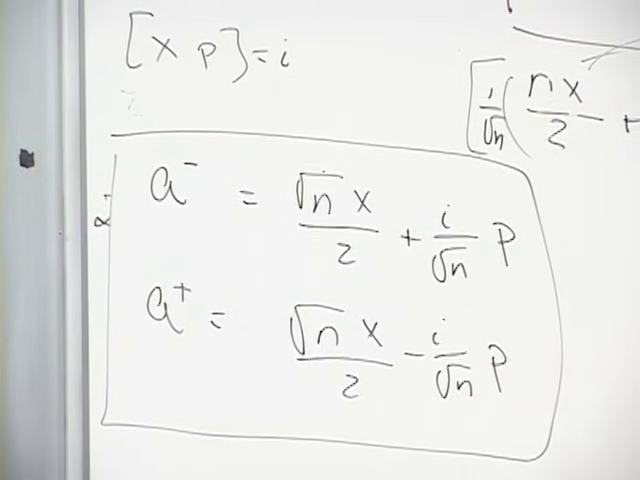
\includegraphics[width=0.82\textwidth]{lecture_03_figure_03.png}
  \caption{\(n\)番目の弦振動子に対する規格化された消滅演算子と生成演算子。}
  \lectureframe{00:12:00}
  \label{fig:l03-ladder-board}
\end{figure}

\subsection{二つの横タワー}

四次元時空において、\(z\)軸に沿って非常に大きな運動量を持つ弦は二つの横座標\(X\)と\(Y\)を持つ。したがって二つの独立な振動子タワーが必要である。\(a_n,a_n^\dagger\)を\(X\)モードに作用させ、\(b_n,b_n^\dagger\)を\(Y\)モードに作用させよう。\eqref{eq:l03-annihilator}--\eqref{eq:l03-creator}を座標について解くと次を得る。

\begin{equation}
  X_n=\frac{a_n+a_n^\dagger}{\sqrt n},
  \qquad
  Y_n=\frac{b_n+b_n^\dagger}{\sqrt n}.
  \label{eq:l03-mode-coordinates}
\end{equation}

\begin{figure}[H]
  \centering
  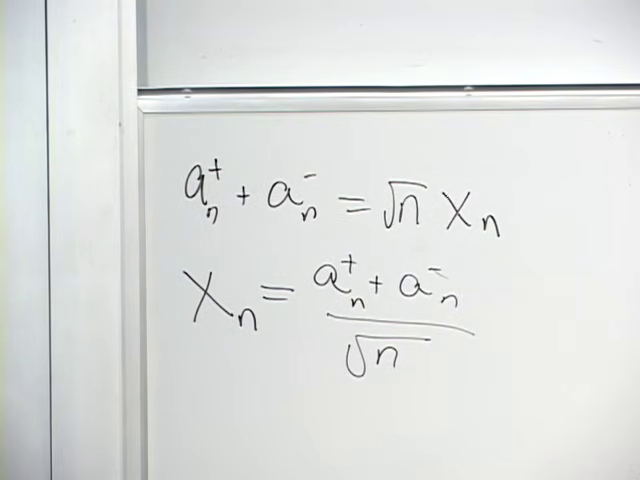
\includegraphics[width=0.78\textwidth]{lecture_03_figure_04.png}
  \caption{モード座標をその生成演算子と消滅演算子で解く。}
  \lectureframe{00:17:05}
  \label{fig:l03-coordinate-operator-board}
\end{figure}

開弦の座標はノイマンモードで展開された。

\begin{align}
  X(\sigma,\tau)
  &=X_{\rm cm}(\tau)
    +\sum_{n=1}^{\infty}X_n(\tau)\cos(n\sigma),
  \label{eq:l03-X-fourier}\\
  Y(\sigma,\tau)
  &=Y_{\rm cm}(\tau)
    +\sum_{n=1}^{\infty}Y_n(\tau)\cos(n\sigma).
  \label{eq:l03-Y-fourier}
\end{align}

端点での傾きが消えるため余弦が現れる。\eqref{eq:l03-mode-coordinates}を代入すると、弦自体が演算子になる。

\begin{align}
  X(\sigma,\tau)
  &=X_{\rm cm}(\tau)
    +\sum_{n=1}^{\infty}
      \frac{a_n(\tau)+a_n^\dagger(\tau)}{\sqrt n}
      \cos(n\sigma),
  \label{eq:l03-X-operator}\\
  Y(\sigma,\tau)
  &=Y_{\rm cm}(\tau)
    +\sum_{n=1}^{\infty}
      \frac{b_n(\tau)+b_n^\dagger(\tau)}{\sqrt n}
      \cos(n\sigma).
  \label{eq:l03-Y-operator}
\end{align}

\begin{figure}[H]
  \centering
  \begin{minipage}[t]{0.48\textwidth}
    \centering
    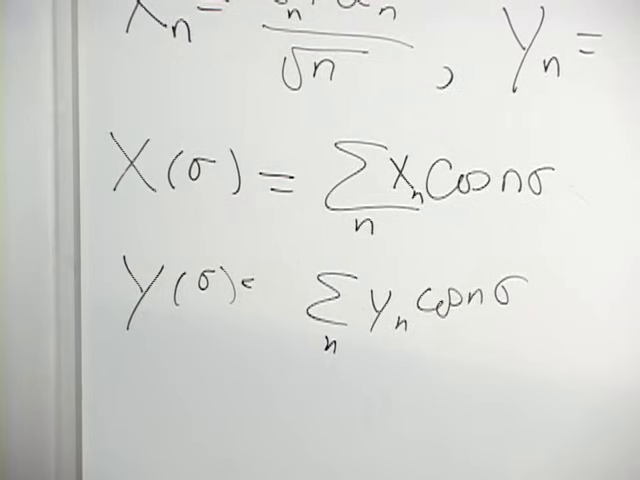
\includegraphics[width=\textwidth]{lecture_03_figure_05.png}
    \par\smallskip\footnotesize (a) 座標モード展開。
  \end{minipage}\hfill
  \begin{minipage}[t]{0.48\textwidth}
    \centering
    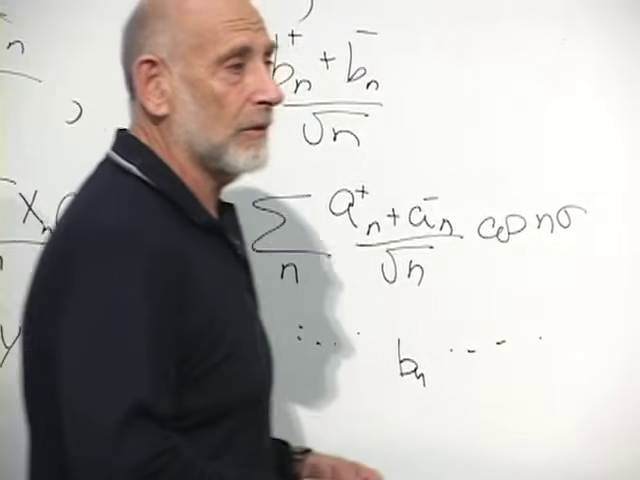
\includegraphics[width=\textwidth]{lecture_03_figure_06.png}
    \par\smallskip\footnotesize (b) はしご演算子を弦座標に代入したもの。
  \end{minipage}
  \caption{量子開弦の形は、そのすべての横振動子演算子から組み立てられる。}
  \lectureframe{00:20:35 and 00:21:05}
  \label{fig:l03-string-coordinate-board}
\end{figure}

\begin{classroomqa}
\audiencequestion{\(X_n\)もまた
\(\sigma\)の関数か。\lecturetimestamp{00:21:48}}
\lecturerresponse{いいえ。\(\sigma\)依存性は完全に
\(\cos(n\sigma)\)の中にある。係数\(X_n\)はその空間的パターンの時間依存振幅であり、したがって\(X_n=X_n(\tau)\)である。}
\end{classroomqa}

\begin{classroomqa}
\audiencequestion{なぜ上昇演算子と下降演算子と呼ばれる演算子は符号が逆に見えるのか。\lecturetimestamp{00:23:13}}
\lecturerresponse{\(ip_n\)の目に見える符号は命名規則ではない。ハミルトニアンとの交換子を計算せよ。
\([H_n,a_n^\dagger]=n a_n^\dagger\)を満たす演算子はエネルギーを上げ、
\([H_n,a_n]=-n a_n\)を満たす演算子はエネルギーを下げる。}
\end{classroomqa}

二つの横タワーは教育的な四次元の描像である。整合的に量子化されたボソン弦は二十六の時空次元を持つので、二つではなく二十四の横振動子族を持つ。以下の論理は変わらない。第一準位の状態の数は、同じ次元における質量ゼロのベクトルの物理的偏極の数と一致しなければならない。

\section{質量のあるスピンと質量ゼロのヘリシティ}

弦の状態にスピンを割り当てる前に、一つの鋭い区別が必要である。スピン\(J\)の質量のある粒子は\(2J+1\)個のスピン状態を持つ。

\begin{equation}
  m_J=-J,-J+1,\ldots,J-1,J.
  \label{eq:l03-massive-spin-multiplet}
\end{equation}

例えば、質量のあるスピン1の粒子は3つの偏極を持ち、質量のあるスピン2の粒子は5つ持つ。その理由は静止系に移ることで理解できる。そこではすべての空間回転が利用可能である。スピン軸を回転させ、元に戻すようにブーストすれば、\(2J+1\)個の成分はすべて同じ相対論的粒子に属する。

質量のない粒子には静止系が存在しない。その不変なスピンラベルはヘリシティ、すなわち運動方向に沿った角運動量である。光子は\(h=+1\)と\(h=-1\)のみを持ち、重力子は\(h=+2\)と\(h=-2\)のみを持つ。スカラーは1つの\(h=0\)状態を持つ。講義では反射対称性を用いて2つのヘリシティを対にする。カイラル理論では、単一の質量のない既約表現が1つのヘリシティのみを担うことがあるため、この対は質量のなさだけから従うのではなく、追加の対称性の主張である。\editorialnote{現代のリトルグループ分類では、1つのヘリシティを持つ質量のない表現が許される。パリティまたは適切なCPT完全な場の内容が、よく知られた光子と重力子の例において反対のヘリシティを与える。}

\begin{figure}[H]
  \centering
  \begin{minipage}[t]{0.45\textwidth}
    \centering
    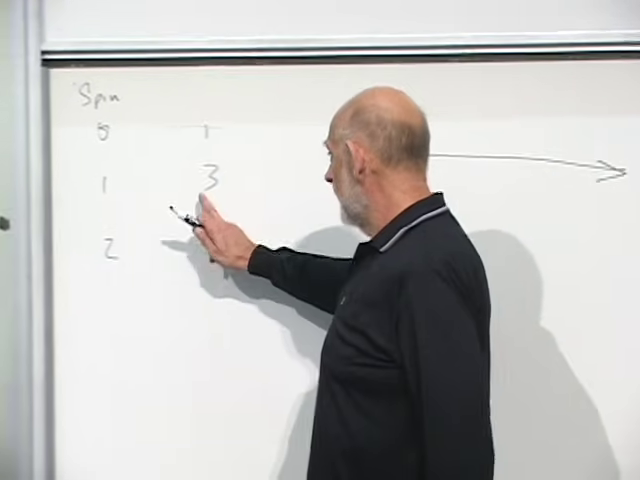
\includegraphics[width=\textwidth]{lecture_03_figure_07.png}
    \par\smallskip\footnotesize (a) 黒板で始められたスピン状態の数え上げ。
  \end{minipage}\hfill
  \begin{minipage}[t]{0.5\textwidth}
    \centering
    \begin{adjustbox}{max width=\linewidth}
    \begin{tabular}{@{}ccc@{}}
      \toprule
      スピン & 質量のある状態 & 質量のないヘリシティ \\
      \midrule
      \(0\) & \(1\) & \(0\) \\
      \(1\) & \(3\) & \(+1,-1\) \\
      \(2\) & \(5\) & \(+2,-2\) \\
      \bottomrule
    \end{tabular}
    \end{adjustbox}
  \end{minipage}
  \caption{質量は静止系を奪い、それとともに中間のスピン射影も奪う。}
  \lectureframe{00:27:40}
  \label{fig:l03-spin-count}
\end{figure}

\subsection{直線偏光と円偏光}

\(z\)に沿って進む光子を考える。その2つの横方向の直線偏光は\(\ket{x}\)と\(\ket{y}\)である。これらはヘリシティ固有状態ではない。円偏光状態は

\begin{align}
  \ket{R}
  &=\frac{1}{\sqrt2}\left(\ket{x}+i\ket{y}\right),
  \label{eq:l03-right-circular}\\
  \ket{L}
  &=\frac{1}{\sqrt2}\left(\ket{x}-i\ket{y}\right),
  \label{eq:l03-left-circular}
\end{align}

であり、ヘリシティは\(+1\)と\(-1\)である（右と左の名付けに用いる規約に依存する）。直線偏光した光子はこれら2つの結果の重ね合わせである。その平均ヘリシティは消えることがあるが、ヘリシティ測定がスピン0の光子を見出すことは決してない。同様に、

\begin{equation}
  \frac{1}{\sqrt2}\left(\ket{x}+\ket{y}\right)
\end{equation}

は単に45度の直線偏光である。

\begin{figure}[H]
  \centering
  \begin{minipage}[t]{0.48\textwidth}
    \centering
    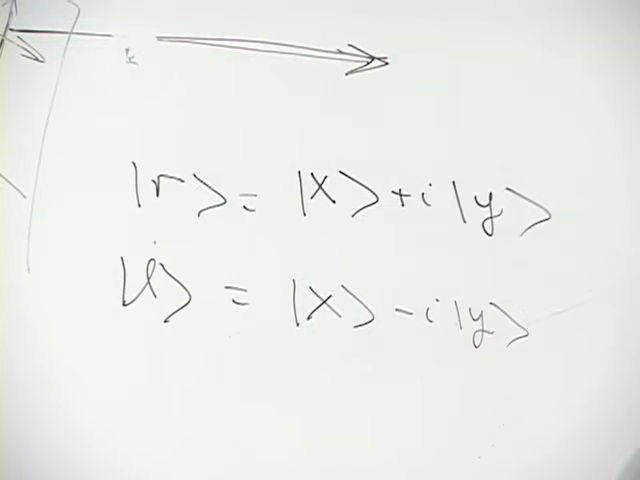
\includegraphics[width=\textwidth]{lecture_03_figure_08.png}
    \par\smallskip\footnotesize (a) 黒板上の円偏光状態。
  \end{minipage}\hfill
  \begin{minipage}[t]{0.48\textwidth}
    \centering
    \begin{adjustbox}{max width=\linewidth}
    \begin{tikzpicture}[>=Latex,scale=0.9]
      \draw[->,thick] (0,0) -- (3.4,0) node[right] {\(z\)};
      \draw[->,blue!70!black,thick] (0,0) -- (0,2.0)
        node[above] {\(x\)};
      \draw[->,orange!85!black,thick] (0,0) -- (-1.4,-1.2)
        node[below left] {\(y\)};
      \draw[red!70!black,thick,->]
        plot[domain=0:320,samples=80]
        ({1.0*cos(\x)},{0.58*sin(\x)+0.4});
      \node[red!70!black] at (1.55,1.25) {circular};
    \end{tikzpicture}
    \end{adjustbox}
  \end{minipage}
  \caption{直線偏光は横方向の基底を与え、円偏光の組み合わせはヘリシティを対角化する。}
  \lectureframe{00:37:45}
  \label{fig:l03-polarization}
\end{figure}

\begin{classroomqa}
\audiencequestion{これはシュテルン--ゲルラッハ実験におけるスピン状態の分離のようなものですか？\lecturetimestamp{00:37:40}}
\lecturerresponse{量子重ね合わせの考え方は同じであるが、光子の場合、直接的な言葉は偏光である。円偏光測定は2つのヘリシティを区別する。ビーム中に縦方向のスピン0の光子は存在しない。}
\end{classroomqa}

重力子はスピン2でこのパターンを繰り返す。スピンの記帳には、模式的には次のように書ける。

\begin{equation}
  \ket{+2}\sim\ket{+1}\otimes\ket{+1},
  \qquad
  \ket{-2}\sim\ket{-1}\otimes\ket{-1}.
  \label{eq:l03-graviton-helicity}
\end{equation}

これは重力子が文字通り2つの光子からできていると言っているのではない。2つの等しいヘリシティが正しいスピン2のヘリシティに加わることを述べているのである。

\begin{classroomqa}
\audiencequestion{2光子の類推は他の量子数にも拡張できますか？\lecturetimestamp{00:41:05}}
\lecturerresponse{構成要素モデルとしては拡張できない。重力の振幅がゲージ理論の振幅の積、あるいは``二乗、''のように見える強力な公式があるが、重力子は依然としてそれ自身の粒子である。この類推が最も信頼できるのは、ここではヘリシティについての主張としてである。\editorialnote{現代のKawai--Lewellen--Tye関係および二重コピー関係は、適切な理論において振幅の主張を精密にするが、重力子を2つの光子の束縛状態に変えるものではない。}}
\end{classroomqa}

\begin{classroomqa}
\audiencequestion{光子は任意の運動量を持ち得るので、粒子に要求される孤立したスペクトルではなく連続スペクトルを持つのではないですか？\lecturetimestamp{00:42:17}}
\lecturerresponse{連続変数は重心運動量である。その運動量を固定して、内部の不変質量を調べる。粒子は孤立した質量準位によって同定され、その全運動量を変えると通常の連続的な分散関係が生じる。}
\end{classroomqa}

\section{開いた弦の最低準位}

ここで弦に戻ることができる。大きな運動量の記述では、有限の内部光円錐エネルギーは不変質量の二乗に比例する。全体の弦のスケールを抑えて、スペクトルを次のように書く。

\begin{equation}
  \begin{aligned}
    M^2
    &=m_0^2
      +\sum_{n=1}^{\infty}n
       \left(N_n^{(a)}+N_n^{(b)}\right),\\
    N_n^{(a)}&=a_n^\dagger a_n,
    \qquad
    N_n^{(b)}=b_n^\dagger b_n.
  \end{aligned}
  \label{eq:l03-open-spectrum}
\end{equation}

振動子の基底状態は次を満たす。

\begin{equation}
  a_n\ket{0}=0,
  \qquad
  b_n\ket{0}=0,
  \qquad n=1,2,\ldots .
  \label{eq:l03-ground-annihilation}
\end{equation}

それは弦が存在しない空の不在ではない。最も励起の少ない量子弦であり、その座標は依然として揺らいでいる。その質量の二乗を\(m_0^2\)としよう。まだ決定されていない。

\begin{figure}[H]
  \centering
  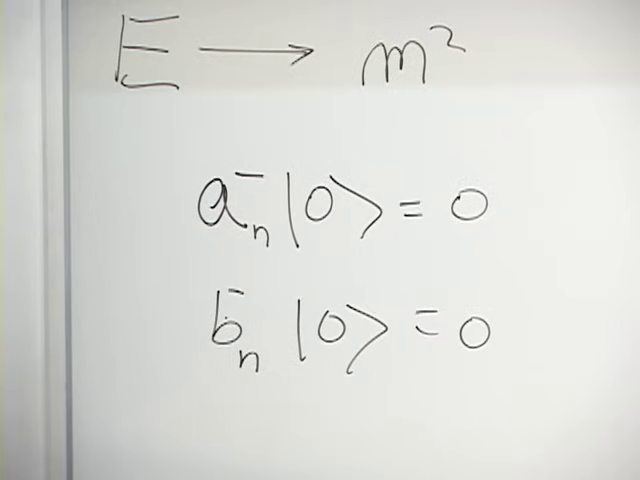
\includegraphics[width=0.78\textwidth]{lecture_03_figure_09.png}
  \caption{開弦の基底状態と、それを定義する消滅条件。}
  \lectureframe{00:45:20}
  \label{fig:l03-ground-state-board}
\end{figure}

最も低コストの励起は\(n=1\)生成演算子を用いる：

\begin{equation}
  a_1^\dagger\ket{0},
  \qquad
  b_1^\dagger\ket{0},
  \qquad
  M^2=m_0^2+1.
  \label{eq:l03-first-level}
\end{equation}

\begin{figure}[H]
  \centering
  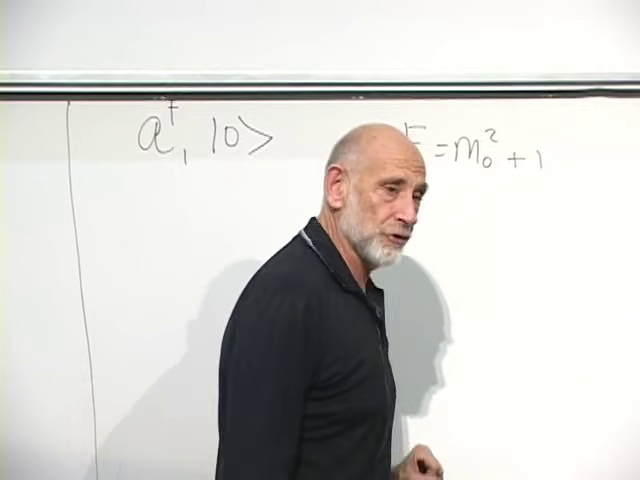
\includegraphics[width=0.78\textwidth]{lecture_03_figure_10.png}
  \caption{二つの縮退した第一準位状態の一方。その質量二乗の増分が黒板に書かれている。}
  \lectureframe{00:49:25}
  \label{fig:l03-first-level-board}
\end{figure}

``1''は、式{eq:l03-first-level}におけるそれは、1ジュールでも1電子ボルトでも1プランク質量でもない。我々は次元を持つ弦のスケールを抑制している。今のところ、それは振動子の質量二乗のはしごにおける1段階を意味する。欠けている単位は次の講義で復元される。

二つの縮退状態の任意の線形結合もまた、この準位の状態である。特に、

\begin{equation}
  \frac{1}{\sqrt2}
  \left(a_1^\dagger\pm i b_1^\dagger\right)\ket{0}
  \label{eq:l03-string-circular-states}
\end{equation}

は円偏光の弦における類似物である。\(x\)-\(y\)平面内の回転の下で、\(a_1^\dagger\)と\(b_1^\dagger\)は横ベクトルの二つの成分として変換する。したがって\eqref{eq:l03-string-circular-states}における結合はヘリシティ\(+1\)と\(-1\)を持つ。

\begin{figure}[H]
  \centering
  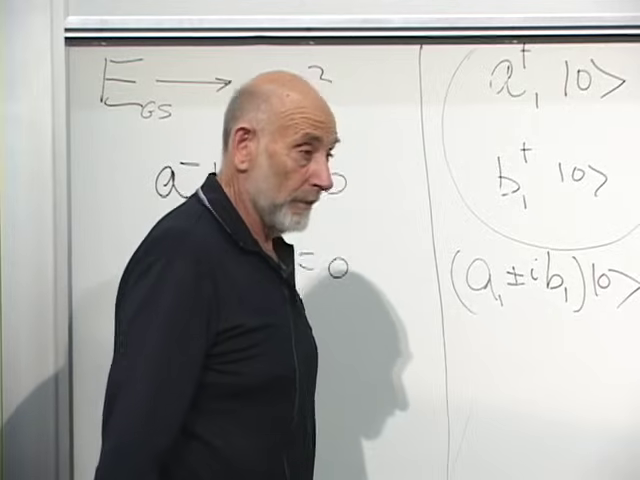
\includegraphics[width=0.82\textwidth]{lecture_03_figure_11.png}
  \caption{基底状態の条件、二つの第一準位励起、およびそれらの円形結合が黒板にまとめられている。}
  \lectureframe{00:56:00}
  \label{fig:l03-level-structure-board}
\end{figure}

縦偏光として働きうる第三の縮退状態は存在しない。もしこれらの二つの状態が非零の質量を持つなら、スピン1の相対論的粒子は三つの偏光を必要とする。ちょうど二つであるなら、その状態は質量ゼロでなければならない。したがって

\begin{equation}
  m_0^2+1=0,
  \qquad
  m_0^2=-1.
  \label{eq:l03-intercept-condition}
\end{equation}

第一準位は光子的である：それは質量ゼロのゲージベクトル状態である。それは電磁気学の光子である必要はない。その最終的なゲージとしての正体は弦模型に依存する。その下の基底状態は負の質量二乗を持つ。それがボソン的開弦のタキオンである。\editorialnote{完全な臨界ボソン弦では、正規順序の切片とローレンツ代数は\(D=26\)に結びついている。講義の二つの横方向の計算は、同じ状態数え上げの議論の四次元的な影である：\(D-2\)個の第一準位振動子状態は、質量ゼロのベクトルの\(D-2\)個の物理的偏光と一致する。}

\begin{classroomqa}
\audiencequestion{なぜ\(m_0^2\)が負であることを気にかけるべきなのか？\lecturetimestamp{00:56:35}}
\lecturerresponse{質量二乗は、我々が真空と呼んできた状態のまわりの二次場ポテンシャルの曲率であるからだ。負の曲率は、この配置が安定な基底状態ではないことを意味する。次の計算がその主張を正確にする。}
\end{classroomqa}

\section{タキオンが本当に意味するもの}

``タキオン''という名は、誤解を招く第一印象を誘う。\(c=1\)として相対論的分散関係から始めよう。

\begin{equation}
  E(p)=\sqrt{p^2+m^2}.
  \label{eq:l03-relativistic-dispersion}
\end{equation}

波束に対して、群速度は

\begin{equation}
  v_g=\frac{dE}{dp}.
  \label{eq:l03-group-velocity}
\end{equation}

これはおなじみの場合を再現する：

\begin{align}
  E_{\rm nr}(p)&=\frac{p^2}{2m},
  &v_g&=\frac{p}{m},
  \label{eq:l03-nr-group-velocity}\\
  E_\gamma(p)&=|p|,
  &|v_g|&=1,
  \label{eq:l03-photon-group-velocity}\\
  E_m(p)&=\sqrt{p^2+m^2},
  &|v_g|&=\frac{|p|}{\sqrt{p^2+m^2}}<1.
  \label{eq:l03-massive-group-velocity}
\end{align}

\begin{figure}[H]
  \centering
  \begin{minipage}[t]{0.48\textwidth}
    \centering
    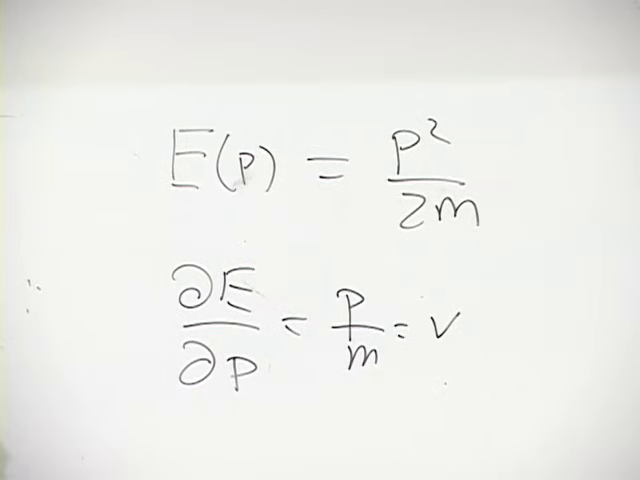
\includegraphics[width=\textwidth]{lecture_03_figure_12.png}
    \par\smallskip\footnotesize (a) 非相対論的群速度。
  \end{minipage}\hfill
  \begin{minipage}[t]{0.48\textwidth}
    \centering
    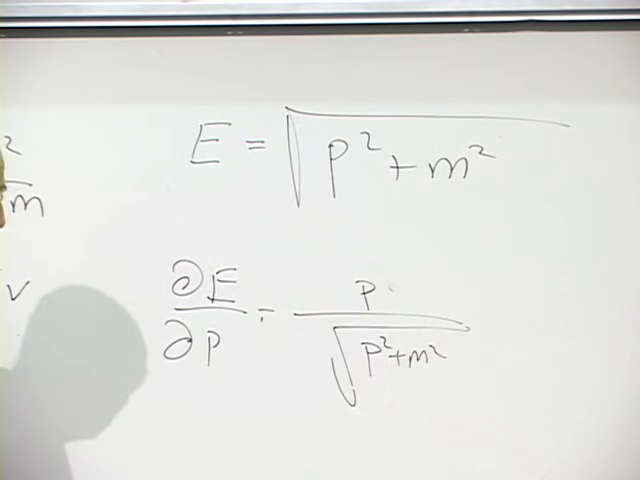
\includegraphics[width=\textwidth]{lecture_03_figure_13.png}
    \par\smallskip\footnotesize (b) 相対論的分散関係とその
    導関数。
  \end{minipage}
  \caption{\(E(p)\)の傾きから伝播速度を読み取る。}
  \lectureframe{01:01:50 and 01:03:15}
  \label{fig:l03-group-velocity-board}
\end{figure}

\(m^2=-\mu^2\)ならば、形式的な表式は

\begin{equation}
  E(p)=\sqrt{p^2-\mu^2},
  \qquad
  v_g=\frac{p}{\sqrt{p^2-\mu^2}},
  \label{eq:l03-formal-tachyon-dispersion}
\end{equation}

となり、平方根が実であるときはいつでも\(|v_g|>1\)を持つ。しかしこれはボソン弦の基底状態の正しい物理的解釈ではない。問題はすでに低運動量で現れ、そこでは振動数が虚数になる。

\subsection{場のポテンシャルの負の曲率}

一次元空間における実スカラー場を考える。

\begin{equation}
  \left(\partial_t^2-\partial_x^2+m^2\right)\phi=0.
  \label{eq:l03-klein-gordon}
\end{equation}

平面波\(\phi\propto e^{-i\omega t+ikx}\)に対して、

\begin{equation}
  \omega^2=k^2+m^2.
  \label{eq:l03-kg-dispersion}
\end{equation}

\begin{figure}[H]
  \centering
  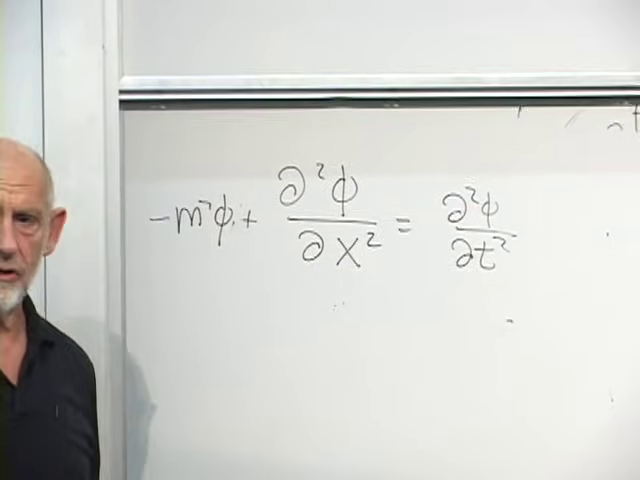
\includegraphics[width=0.82\textwidth]{lecture_03_figure_14.png}
  \caption{負の質量二乗の背後にある不安定性を露わにするために用いられるKlein--Gordon方程式。}
  \lectureframe{01:06:40}
  \label{fig:l03-klein-gordon-board}
\end{figure}

保存する二次エネルギーは

\begin{equation}
  \mathcal E
  =\frac12\int dx\,
  \left[
    \dot\phi^{\,2}
    +(\partial_x\phi)^2
    +m^2\phi^2
  \right].
  \label{eq:l03-field-energy}
\end{equation}

\begin{figure}[H]
  \centering
  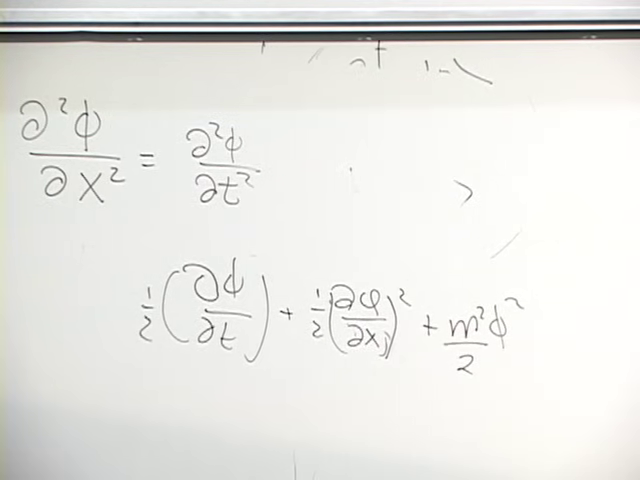
\includegraphics[width=0.82\textwidth]{lecture_03_figure_15.png}
  \caption{スカラー場のエネルギー。質量項がポテンシャルの局所的な曲率を与えている。}
  \lectureframe{01:08:10}
  \label{fig:l03-field-energy-board}
\end{figure}

\(m^2>0\)に対して、局所ポテンシャル\(V(\phi)=\tfrac12m^2\phi^2\)はすり鉢である。配置\(\phi=0\)はその底に位置する。\(m^2=-\mu^2\)に対して、同じ点は逆さにしたすり鉢の頂上である。方程式\eqref{eq:l03-kg-dispersion}は次のようになる。

\begin{equation}
  \omega^2=k^2-\mu^2.
  \label{eq:l03-tachyonic-modes}
\end{equation}

\(k^2<\mu^2\)を持つモードは

\begin{equation}
  \omega=\pm i\sqrt{\mu^2-k^2},
  \qquad
  \phi_k(t)\propto
  e^{\pm\sqrt{\mu^2-k^2}\,t}.
  \label{eq:l03-growing-mode}
\end{equation}

一方の枝は指数関数的に成長する。したがって、いわゆる真空は不安定である：任意に小さな長波長の擾乱が場を\(\phi=0\)から遠ざける。これがスペクトル中のタキオンが意味するものである。

\subsection{直立振り子の鎖}

結合した振り子の列は、この区別を目に見える形にする。すべての振り子を直立させる。一様な配置は存在するが、それは位置エネルギーの極大で釣り合っている。一つの振り子をわずかに押すと、それは倒れ、隣の振り子を引っ張る。倒れる振り子の前線は、結合によって定まる有限の信号速度で鎖の中を広がっていく。

\begin{figure}[H]
  \centering
  \begin{minipage}[t]{0.48\textwidth}
    \centering
    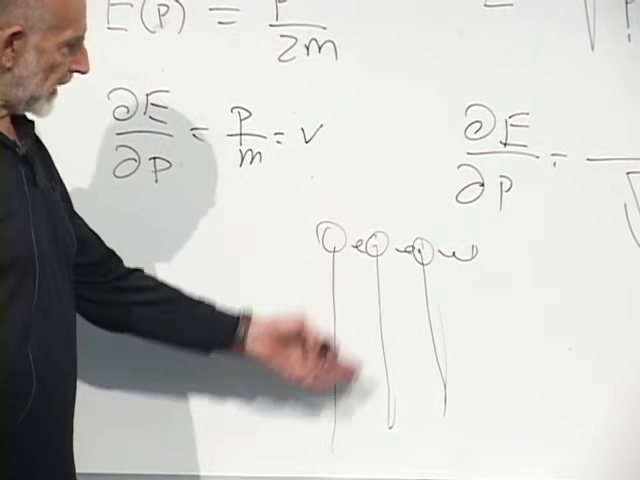
\includegraphics[width=\textwidth]{lecture_03_figure_16.png}
    \par\smallskip\footnotesize (a) 板上の結合した直立振り子模型。
  \end{minipage}\hfill
  \begin{minipage}[t]{0.48\textwidth}
    \centering
    \begin{adjustbox}{max width=\linewidth}
    \begin{tikzpicture}[>=Latex,scale=0.78]
      \draw[thick] (-0.3,0) -- (6.3,0);
      \foreach \x/\a in {0/0,1/0,2/8,3/28,4/55,5/72,6/78}{
        \fill (\x,0) circle (0.06);
        \draw[thick] (\x,0) -- ++({90-\a}:1.25);
        \fill[blue!65!black]
          ($(\x,0)+({90-\a}:1.25)$) circle (0.11);
      }
      \draw[red!70!black,->,thick] (1.7,-0.45) -- (4.6,-0.45)
        node[midway,below] {falling front};
    \end{tikzpicture}
    \end{adjustbox}
  \end{minipage}
  \caption{線形化スペクトルが負の質量二乗を含んでいても、不安定性は系の中を因果的に広がる。}
  \lectureframe{01:10:40}
  \label{fig:l03-pendulum-instability}
\end{figure}

この機構のどこにも、制御された信号が因果的前線を追い越すことは許されない。タキオン的モードは、超光速の安定な伝令ではなく、悪い展開点を診断するものである。\editorialnote{局所的な相対論的場の方程式に対して、前線速度は因果的速度のままである。実の高\(k\)分枝の形式的な群速度は、不安定な真空を超光速通信路に変えるものではない。}

\begin{classroomqa}
\audiencequestion{いま見つかった質量ゼロの状態は、弦理論が予言する重力子そのものですか。\lecturetimestamp{01:14:27}}
\lecturerresponse{いいえ。それは開いた弦の二つの偏極をもつスピン1の状態であり、したがってゲージボソン的なものである。重力子は閉じた弦のスピン2の励起である。}
\end{classroomqa}

\begin{classroomqa}
\audiencequestion{逆さまのポテンシャルは数学的に許されるのですか。また、系は落下した後どこで落ち着くのですか。\lecturetimestamp{01:15:17}}
\lecturerresponse{それは完全に正当な局所近似であるが、それ自体では基底状態をもたない。エネルギーが下に有界でないからである。より完全なポテンシャルは再び上向きに曲がり、より低い極小をもつかもしれない。そのとき系はその安定な配置へ向かって転がるか凝縮する。}
\end{classroomqa}

通常のボソン弦はまさにこの欠陥をもつ。そのより高い振動子状態はスペクトルの一部であり続けるが、それらは不安定な背景の励起である。整合的な超弦理論は、その安定なセクターにおいて開いた弦のタキオンを取り除きつつ、質量ゼロおよび質量をもつ弦の励起を保持する。

\begin{classroomqa}
\audiencequestion{開いた弦の状態の他の性質も、その二つの偏極と同じように光子に一致しますか。\lecturetimestamp{01:17:07}}
\lecturerresponse{その状態は質量ゼロのゲージボソンとして振る舞う。その詳細な電荷の割り当て、放射則、および正体は弦模型に依存するので、ただちに電磁気学と同一視するのではなく、光子的なものと呼ぶべきである。それらの相互作用の性質は後で展開される。}
\end{classroomqa}

\section{弦はどのように相互作用するか}

自由なスペクトルは理論の半分にすぎない。弦はまた結合したり分裂したりする。まず、励起した自由な弦が角運動量を運びうることを思い出すと有用である。まっすぐな回転する弦はその重心のまわりで回転し、そのエネルギーと角運動量はよく知られた弦的軌跡に沿ってともに増大する。

\begin{figure}[H]
  \centering
  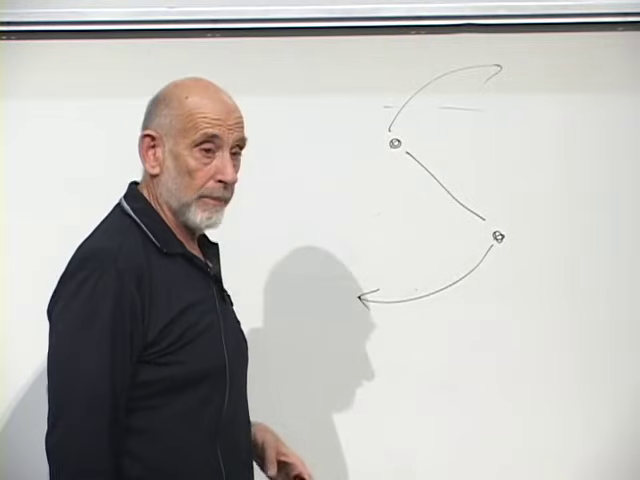
\includegraphics[width=0.72\textwidth]{lecture_03_figure_17.png}
  \caption{重心点のまわりに描かれた回転する開いた弦。}
  \lectureframe{01:19:30}
  \label{fig:l03-rotating-string-board}
\end{figure}

\begin{classroomqa}
\audiencequestion{自由な弦は、一つの固定された端点のまわりで端から端へ回転できますか。\lecturetimestamp{01:20:02}}
\lecturerresponse{錨がなければできない。自由な孤立系はその重心のまわりで回転する。端点が別の物体やブレーンに付着していれば、複合系は異なる中心のまわりで回転できる。ちょうど電子と原子核がそれらの共通の重心のまわりを回り、はるかに重い原子核がほとんど固定して見えるのと同じである。}
\end{classroomqa}

\subsection{開いた弦の頂点}

開いた弦では、素過程の相互作用は二つの端点が同じ時空点で出会うときに起こる。それらが結合して一つの弦を形成する振幅\(g_s\)がある。履歴を逆にたどると、一つの弦が二つに分裂する振幅が得られる。概略的には、

\begin{equation}
  \text{open}+\text{open}
  \quad\rightleftarrows\quad
  \text{open}.
  \label{eq:l03-open-joining}
\end{equation}

\begin{figure}[H]
  \centering
  \begin{minipage}[t]{0.48\textwidth}
    \centering
    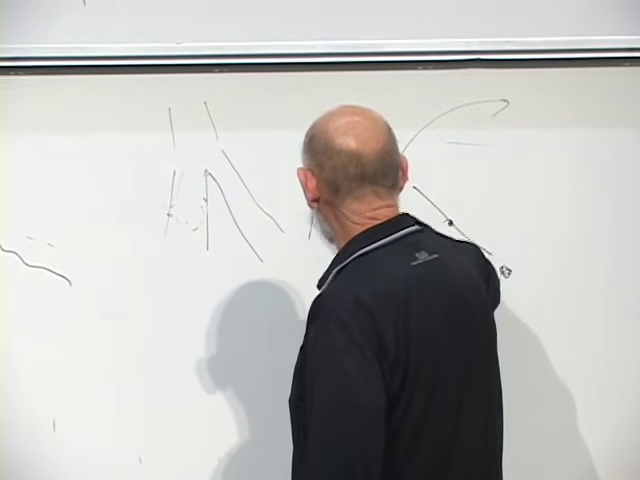
\includegraphics[width=\textwidth]{lecture_03_figure_18.png}
    \par\smallskip\footnotesize (a) 板上の結合の履歴。
  \end{minipage}\hfill
  \begin{minipage}[t]{0.48\textwidth}
    \centering
    \begin{tikzpicture}[>=Latex,scale=0.9]
      \draw[->] (0,-2.1) -- (0,2.2) node[above] {time};
      \draw[blue!70!black,thick] (-2,-1.6) .. controls (-1.3,-0.9)
        and (-0.7,-0.35) .. (0,0);
      \draw[blue!70!black,thick] (2,-1.6) .. controls (1.3,-0.9)
        and (0.7,-0.35) .. (0,0);
      \draw[orange!85!black,thick] (0,0) .. controls (0.25,0.7)
        and (-0.15,1.25) .. (0.15,1.9);
      \fill[red!70!black] (0,0) circle (0.09);
      \node[right] at (0.12,0) {\(g_s\)};
    \end{tikzpicture}
  \end{minipage}
  \caption{端点の結合は、局所的な粒子の相互作用頂点の弦版であり、時間反転が分裂を与える。}
  \lectureframe{01:24:05}
  \label{fig:l03-open-vertex}
\end{figure}

結合は振幅である。一つの指定された素過程に対して、対応する確率は\(|g_s|^2\)の次数から始まり、位相空間因子と規格化因子は完全な計算によって与えられる。したがって\(g_s\)を``確率''と呼ぶのは非公式な略記である。振幅と確率を区別しておくことで、誤った二乗を避けられる。

この相互作用は、外部の弦がたまたま振動しているか、回転しているか、あるいは他の振動子状態にあるかには依存しない。それらの状態は詳細な行列要素を変えるが、同じ局所的な接合規則が用いられる。

\subsection{開弦は自ら閉じることができる}

1本の開弦の2つの端点が出会うとしよう。接合規則は、それらが同じ弦に属することを知り得ない。それらは融合して閉じたループを生成し得る：

\begin{equation}
  \text{open}\longrightarrow\text{closed}.
  \label{eq:l03-self-closing}
\end{equation}

\begin{figure}[H]
  \centering
  \begin{minipage}[t]{0.48\textwidth}
    \centering
    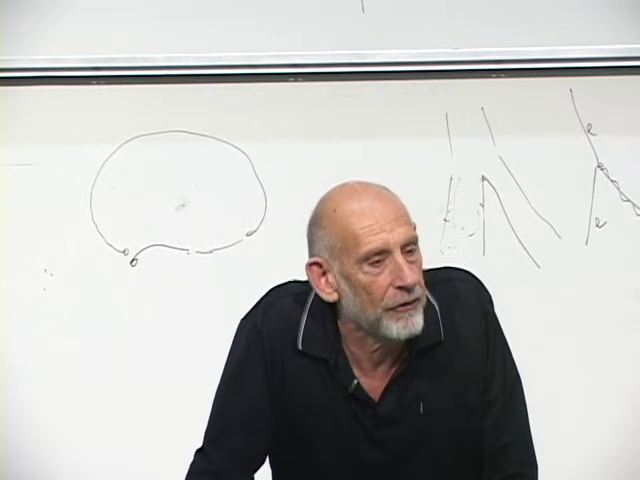
\includegraphics[width=\textwidth]{lecture_03_figure_19.png}
    \par\smallskip\footnotesize (a) 開弦がその端点を近づける。
  \end{minipage}\hfill
  \begin{minipage}[t]{0.48\textwidth}
    \centering
    \begin{tikzpicture}[>=Latex,scale=0.92]
      \draw[blue!70!black,thick]
        (-2,0) .. controls (-1.2,1.5) and (1.2,1.5) .. (2,0);
      \fill[red!70!black] (-2,0) circle (0.08);
      \fill[red!70!black] (2,0) circle (0.08);
      \draw[->,thick] (-0.45,-0.45) -- (0.45,-0.45);
      \draw[orange!85!black,thick] (0,-1.55) ellipse (1.15 and 0.58);
      \node at (0,-2.25) {closed string};
    \end{tikzpicture}
  \end{minipage}
  \caption{相互作用する開弦は必然的に閉弦を生成する。}
  \lectureframe{01:27:20}
  \label{fig:l03-open-becomes-closed}
\end{figure}

これは任意の装飾ではない。相互作用する開弦のいかなる理論も、閉弦状態を含まなければならない。逆の過程では、許された端点と境界条件が存在するとき、閉弦が開弦へと開くことができる。

\begin{classroomqa}
\audiencequestion{弦が融合または分裂するとき、その振動子エネルギーは変化するのか、また理論はそれがどのように変化するかを決定するのか。\lecturetimestamp{01:28:05}}
\lecturerresponse{はい。エネルギーと運動量は過程全体で保存されるが、励起は出ていく弦の間で再分配され得る。相互作用頂点と外部波動関数が遷移振幅を決定する。}
\end{classroomqa}

\subsection{閉弦は開くことなく相互作用できる}

含意は一方通行である。相互作用する開弦は閉弦を必要とするが、理論は閉弦のみから始まってもよい。2つの閉じたループは接触し、再結合して1つの閉じたループになり得る。逆の履歴は1つのループを2つに分裂させる。開いた端点が現れる必要はない。

\begin{figure}[H]
  \centering
  \begin{minipage}[t]{0.48\textwidth}
    \centering
    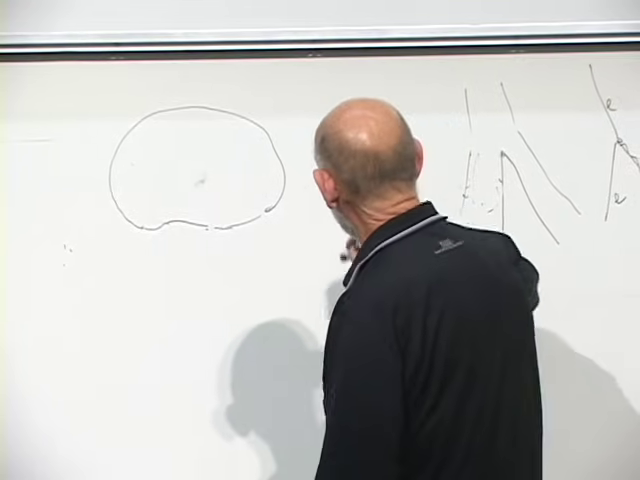
\includegraphics[width=\textwidth]{lecture_03_figure_20.png}
    \par\smallskip\footnotesize (a) 黒板上での閉弦の融合。
  \end{minipage}\hfill
  \begin{minipage}[t]{0.48\textwidth}
    \centering
    \begin{tikzpicture}[>=Latex,scale=0.88]
      \draw[blue!70!black,thick] (-1.35,0) circle (0.75);
      \draw[blue!70!black,thick] (1.35,0) circle (0.75);
      \draw[->,thick] (-0.35,-1.15) -- (0.35,-1.15);
      \draw[orange!85!black,thick] (0,-2.3) ellipse (1.35 and 0.68);
      \node at (0,1.2) {closed \(+\) closed};
      \node at (0,-3.25) {closed};
    \end{tikzpicture}
  \end{minipage}
  \caption{閉弦はそれ自身の接合および分裂の相互作用を持ち、開弦状態を経由する必要はない。}
  \lectureframe{01:29:05}
  \label{fig:l03-closed-fusion}
\end{figure}

\begin{classroomqa}
\audiencequestion{理論が閉弦から始まるならば、開弦もまた含まなければならないか。\lecturetimestamp{01:28:35}}
\lecturerresponse{いいえ。閉弦は全体を通じて閉じたままで再結合によって相互作用できる。開弦は、許された端点やブレーンなどの追加の境界データを必要とする。}
\end{classroomqa}

\section{重力を避けられない理由}

閉弦の振動子計算は開弦のものと並行するが、独立な左巻きおよび右巻きの励起が存在する。それらの最低の非自明な整合したレベルは、質量ゼロのスピン2状態を含む。その状態はグラビトンのヘリシティを持つ。したがって、整合する相互作用する閉弦理論はすべて重力を含む。

\begin{classroomqa}
\audiencequestion{なぜ開弦のレベルが光子様でなければならなかったのと同様に、最低の閉弦励起はグラビトンでなければならないのか。
\lecturetimestamp{01:30:59}}
\lecturerresponse{答えは同じ種類の状態の数え上げであり、今度は左巻きおよび右巻きの振動子ベクトルを伴う。それらのテンソル積は、質量ゼロの対称トレースレススピン2偏極を含む。明示的な閉弦スペクトルは次に計算されるであろう。この段階での要点は、その状態の必然性である。}
\end{classroomqa}

開弦と閉弦は互いに相互作用することもできる。閉じたループは開弦に出会い吸収されて、より大きいか異なる励起状態の開弦を残し得る。逆に、開弦は閉じたループを放射し得る。粒子レベルでは、これは物質によるグラビトンの放出または吸収である。

\begin{figure}[H]
  \centering
  \begin{minipage}[t]{0.48\textwidth}
    \centering
    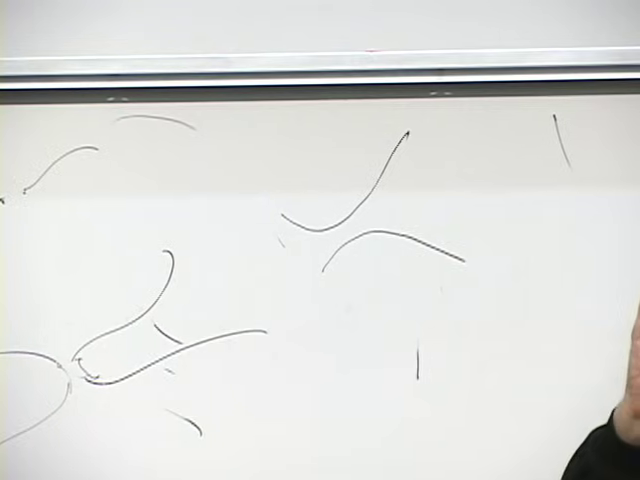
\includegraphics[width=\textwidth]{lecture_03_figure_21.png}
    \par\smallskip\footnotesize (a) 弦の断片の局所的な再結合。
  \end{minipage}\hfill
  \begin{minipage}[t]{0.48\textwidth}
    \centering
    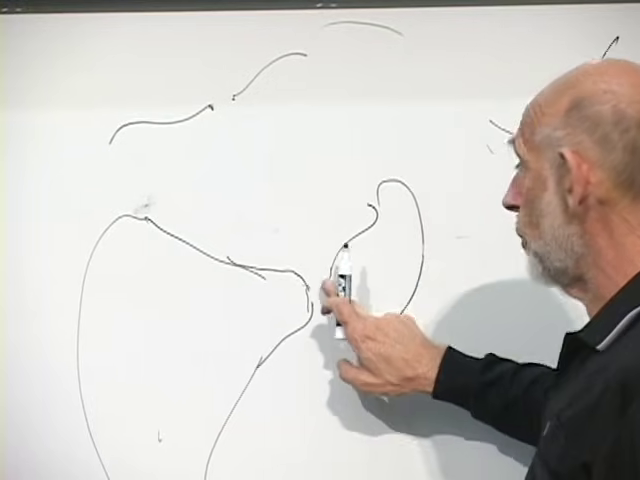
\includegraphics[width=\textwidth]{lecture_03_figure_22.png}
    \par\smallskip\footnotesize (b) 閉じたループが開いた弦に付着する。
  \end{minipage}
  \caption{混合した開いた弦--閉じた弦の相互作用と、重力子交換の普遍的可能性の背後にある黒板の図。}
  \lectureframe{01:33:10 and 01:34:35}
  \label{fig:l03-mixed-interactions-board}
\end{figure}

\begin{figure}[H]
  \centering
  \begin{tikzpicture}[>=Latex,scale=0.88]
    \draw[blue!70!black,thick]
      (-3,-0.5) .. controls (-1.7,-0.1) and (-0.8,0.2) .. (0,0);
    \draw[blue!70!black,thick]
      (0,0) .. controls (0.9,0.3) and (2.0,0.1) .. (3,0.55);
    \draw[orange!85!black,thick] (-0.8,1.55) ellipse (0.75 and 0.45);
    \draw[->,red!70!black,thick] (-0.45,1.15) -- (-0.05,0.35);
    \node[blue!70!black] at (-2.2,-0.95) {open string};
    \node[orange!85!black] at (-0.8,2.25) {closed string};
    \node at (1.75,-0.5) {excited open string};
  \end{tikzpicture}
  \caption{開弦による閉弦の吸収の、時空に依らない明快な模式図。}
  \label{fig:l03-mixed-interaction-redraw}
\end{figure}

グラビトンはすべての弦状態に結合し得る。なぜなら、すべての弦はエネルギーと運動量を運び、接合規則が閉弦の交換を許すからである。これが重力の普遍性の弦理論的起源である。

\begin{classroomqa}
\audiencequestion{閉じた弦が開いた弦になることはできるのか、あるいは端点の規則を破ることなく開いた弦に結合できるのか。\lecturetimestamp{01:31:20}}
\lecturerresponse{両方のセクターを含む理論では、閉じた弦は開いた弦に付着してその状態を変えることができる。孤立した閉じた弦が単に開くことができるかどうかは、その理論が許容される端点を供給するかどうかに依存する。局所的な再結合の規則は同じままである。}
\end{classroomqa}

\begin{classroomqa}
\audiencequestion{閉じたループは永久的に連結したり結び目を作ったりすることができるのか。\lecturetimestamp{01:35:10}}
\lecturerresponse{弱結合では弦はほとんど透明である。すなわち、小さな再結合振幅が作用しない限り、弦は互いを通り抜けることができる。したがって、連結や結び目はしばらくの間持続しうるが、許された弦の相互作用が起こるとトポロジーは変化しうる。}
\end{classroomqa}

\begin{classroomqa}
\audiencequestion{相互作用の確率は弦の状態や速さに依存しないのか。\lecturetimestamp{01:36:09}}
\lecturerresponse{局所的な結合は同じパラメータであるが、全遷移確率は波動関数にも、また関連する部分がどれだけ長く接触しているかにも依存する。速い遭遇は一般に遅いものよりも短い相互作用時間しか与えない。}
\end{classroomqa}

\section{依然として欠けているスケールと結合}

二つの帳尻合わせが意図的に先延ばしにされてきた。第一に、\(X\) は長さであるのに対し \(a_n\) は無次元であるから、\eqref{eq:l03-mode-coordinates} における比例関係は長さのスケールを含まなければならない。第二に、振動子の準位を上げることは、無次元の数を物理的な質量の二乗に文字通り加えることはできない。弦の長さ \(\ell_s\)、あるいは同等にレッジェ傾き \(\alpha'\sim\ell_s^2\) を復元すれば、欠けていた次元が供給される。

\begin{equation}
  M^2\sim\frac{1}{\alpha'}(N-a).
  \label{eq:l03-dimensional-spectrum}
\end{equation}

正確な規約と規格化は次の講義で固定される。

\begin{classroomqa}
\audiencequestion{弦の長さの単位と、一つの生成演算子によって加えられる質量を定めるものは何か。\lecturetimestamp{01:37:03}}
\lecturerresponse{次元を持つ定数が抑圧されてきた。それは弦のスケールであり、通常 \(\ell_s\) または \(\alpha'\) と書かれる。振動子演算子は無次元であり、そのスケールの冪がそれらの準位数を物理的な長さ、張力、質量の二乗に変換する。}
\end{classroomqa}

第二のパラメータは弦の結合 \(g_s\) である。最も単純な議論では、それは結合と分裂を支配する一つの普遍的な数である。より豊かな模型では、端点が異なるラベルを担うことができ、弦は接合部で出会うことができる。Y字型の配置は三本のフラックス管が出会うことの弦における類似物であり、古いハドロン的描像では三クォークバリオンと関連づけられるのに対し、単一の開いた線分はクォーク--反クォーク中間子に似ている。

\begin{classroomqa}
\audiencequestion{異なる弦の端点は異なる結合確率を持ちうるのか。\lecturetimestamp{01:39:31}}
\lecturerresponse{最も単純な模型は一つの結合を用いる。より精巧な理論では端点に電荷や境界ラベルを付与し、選択則がどの結合が許されるかを決める。詳細な構成は先延ばしにされるが、普遍的な局所結合の考え方は生き残る。}
\end{classroomqa}

\begin{classroomqa}
\audiencequestion{弦は縦に分裂したり、Y字型の接合部を形成したりすることができるのか。\lecturetimestamp{01:40:01}}
\lecturerresponse{一部の弦の系は実際に接合部を許容する。それらは今描いた通常の二端点分裂過程ではないが、理論が両立する弦の電荷を持つときに生じる。中間子--バリオンのフラックス管の類推は、この区別の有用な描像である。}
\end{classroomqa}

\begin{classroomqa}
\audiencequestion{時空の次元数を変えると相互作用の結合は変わるのか。\lecturetimestamp{01:42:25}}
\lecturerresponse{次元はスペクトル、位相空間、およびコンパクト化後に得られる有効結合を変える。基本的な弦の結合は依然として摂動展開を組織するが、その低次元での現れ方は余剰次元の幾何と体積に依存する。}
\end{classroomqa}

\begin{classroomqa}
\audiencequestion{自由な弦がそもそも運動するのは重力のせいなのか。\lecturetimestamp{01:43:17}}
\lecturerresponse{運動を維持するのに力は必要ない。初期の位置と速度が自由解を指定し、慣性がそれを前へ運ぶ。重力や別の力はその運動を変える。初期条件の原因を問うことは別の問題であり、局所的な運動方程式の一部ではない。}
\end{classroomqa}

したがって我々は三つの連関した結論に到達した。開いた弦を量子化すると、その第一励起準位に質量ゼロのベクトルが生じる。その下のボソン的基底状態は不安定である。そして相互作用は必然的に閉じた弦を導入し、そのスペクトルは重力を含む。次の課題は、欠けているスケールを復元し、閉じた弦の量子化を陽に実行することである。
